\documentclass{beamer}

%%%%%%%%%%%%%Solarized Theme%%%%%%%%%%%%%%%
\usecolortheme[dark,accent=cyan]{solarized}
\beamertemplatenavigationsymbolsempty

%%%%%Packages%%%%%
\usepackage{graphicx}
\usepackage{hyperref}
\usepackage{colortbl, xcolor}
\usepackage{booktabs}
\usepackage{standalone}

\usepackage{tikz}
\usetikzlibrary{calc}

\usepackage{minted}

\definecolor{DarkGray}{gray}{0.1}
\definecolor{DarkGray}{gray}{0.1}
\usemintedstyle{native}

%%%%%%Title%%%%%%%%
\title{\textcolor{orange}{Introduction to Time Series}}
\author{Nikoleta Glynatsi}
\date{Mathematics \& CUBRIC workshop}

\begin{document}

\maketitle

\begin{frame}
    \begin{center}
    
\includegraphics[width=0.24\textwidth]{static/cardiff_uni_logo.jpg}\hspace{10pt}
    
\includegraphics[width=0.24\textwidth]{static/ssi-logo.png}
    \end{center}
\end{frame}

\begin{frame}
    \begin{center}
    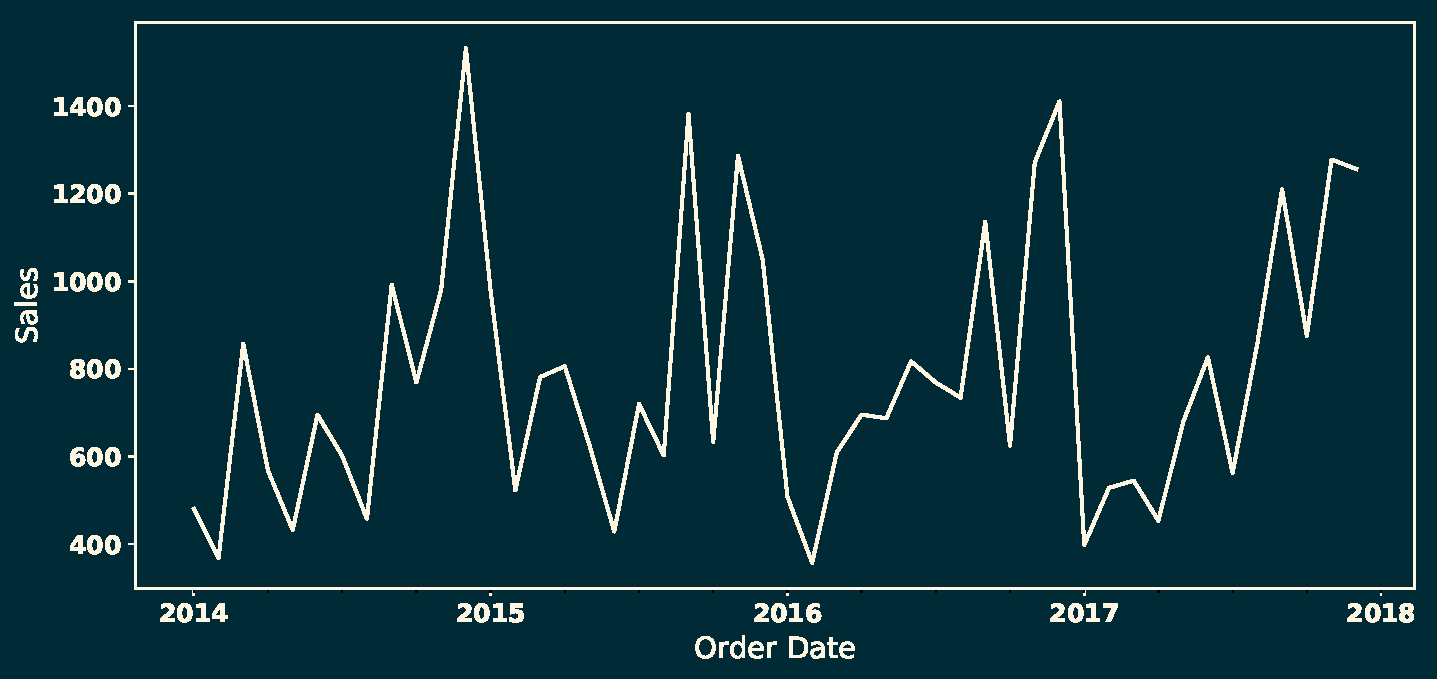
\includegraphics[width=\textwidth]{static/sales.pdf}\vspace{1cm}

    Superstore Sales
    \end{center}
\end{frame}

\begin{frame}
    \begin{center}
        \includestandalone{static/components}
    \end{center}
\end{frame}

\begin{frame}
    \begin{center}
    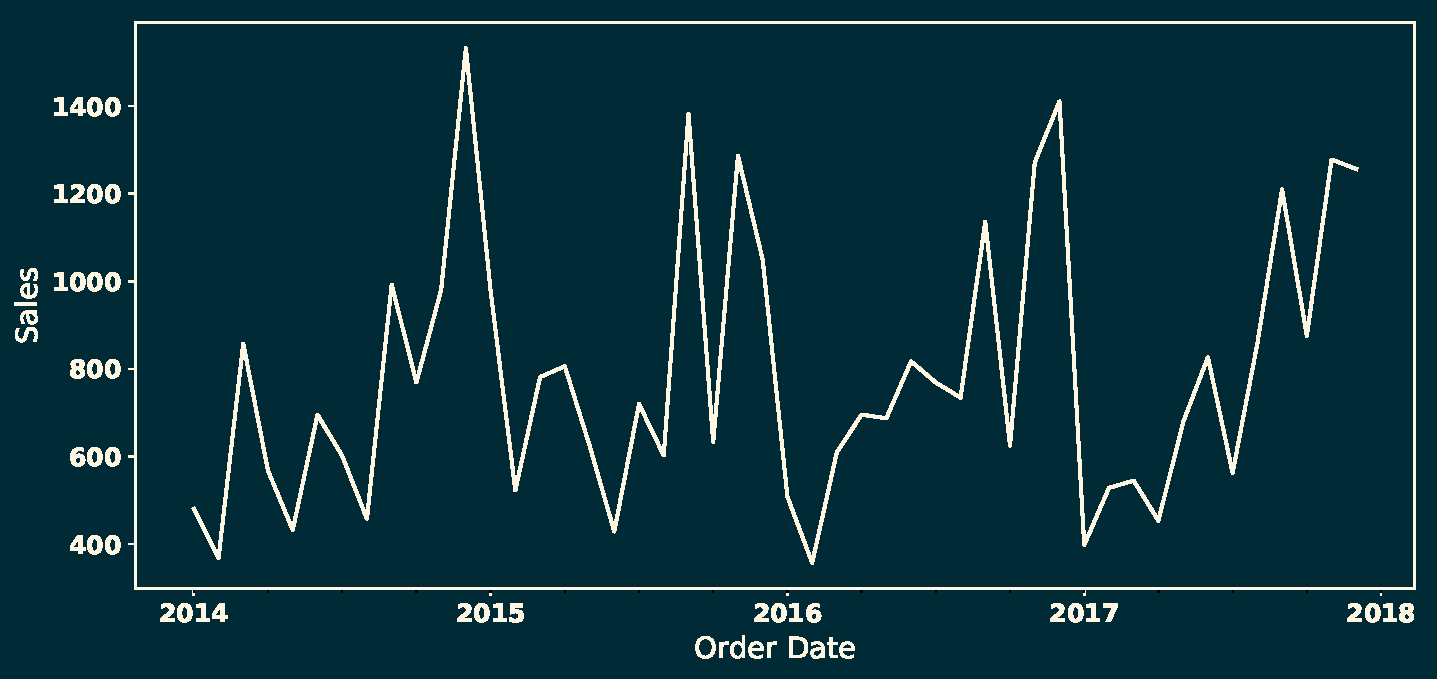
\includegraphics[width=.7\textwidth]{static/sales.pdf}
    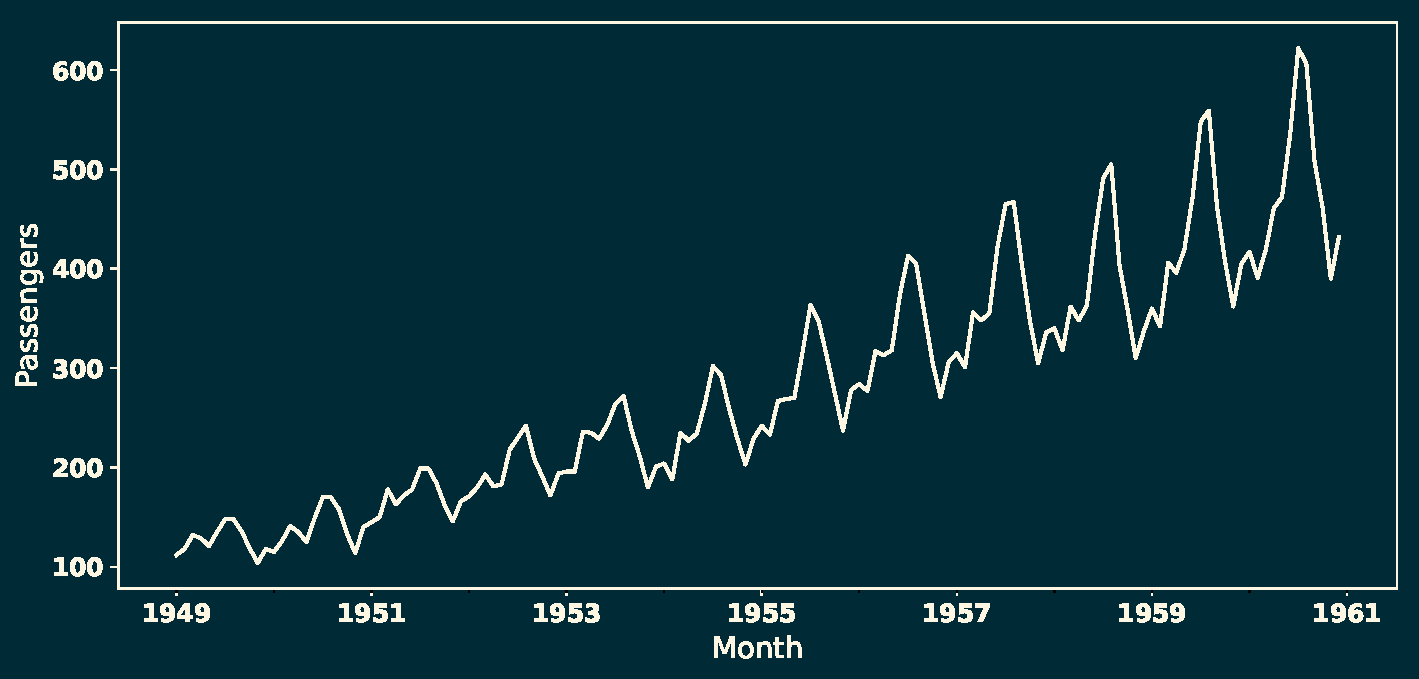
\includegraphics[width=.7\textwidth]{static/airline_passengers.pdf}
    \end{center}
\end{frame}

\begin{frame}
    \begin{center}
    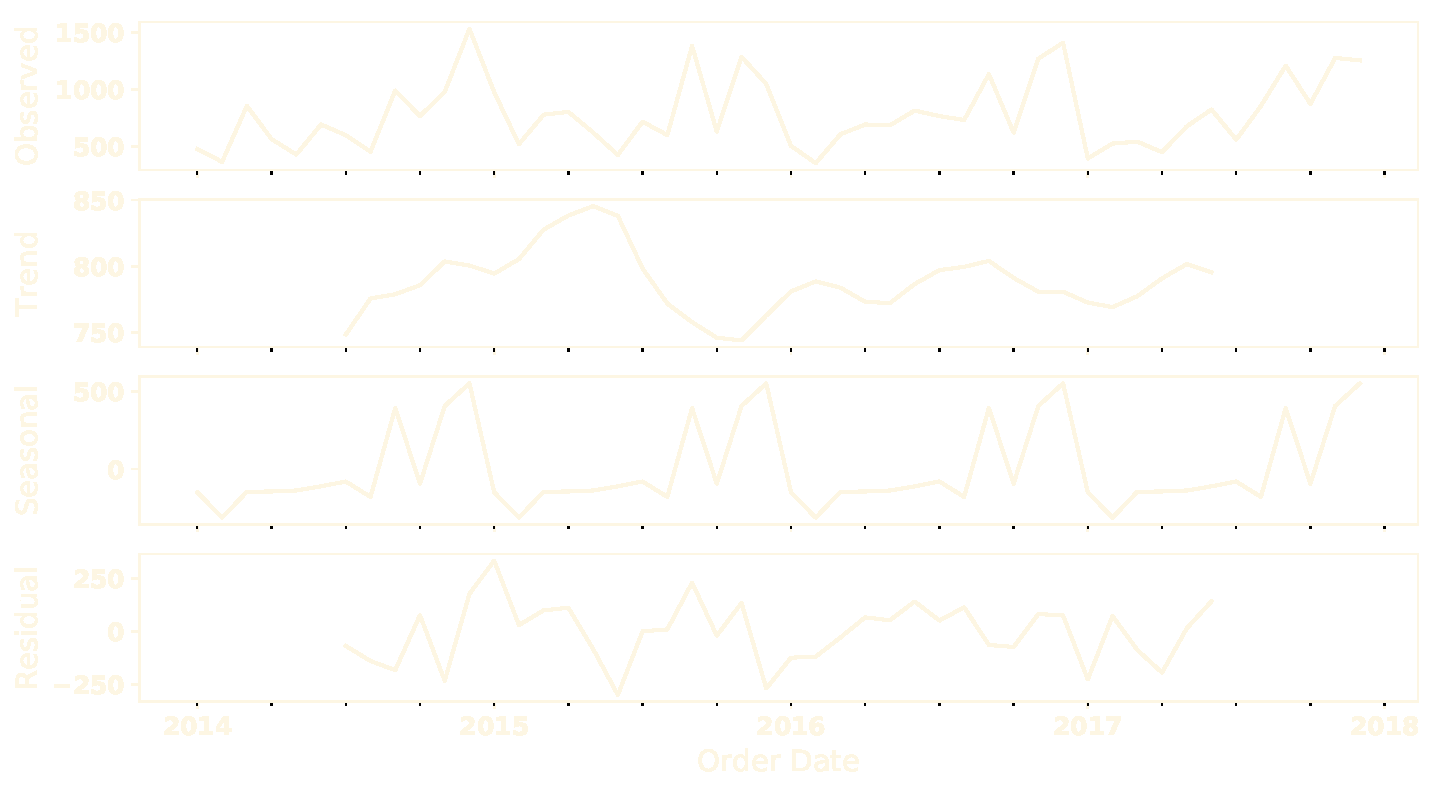
\includegraphics[width=\textwidth]{static/decomposition.pdf}
    \end{center}
\end{frame}

\begin{frame}
    \begin{center}
    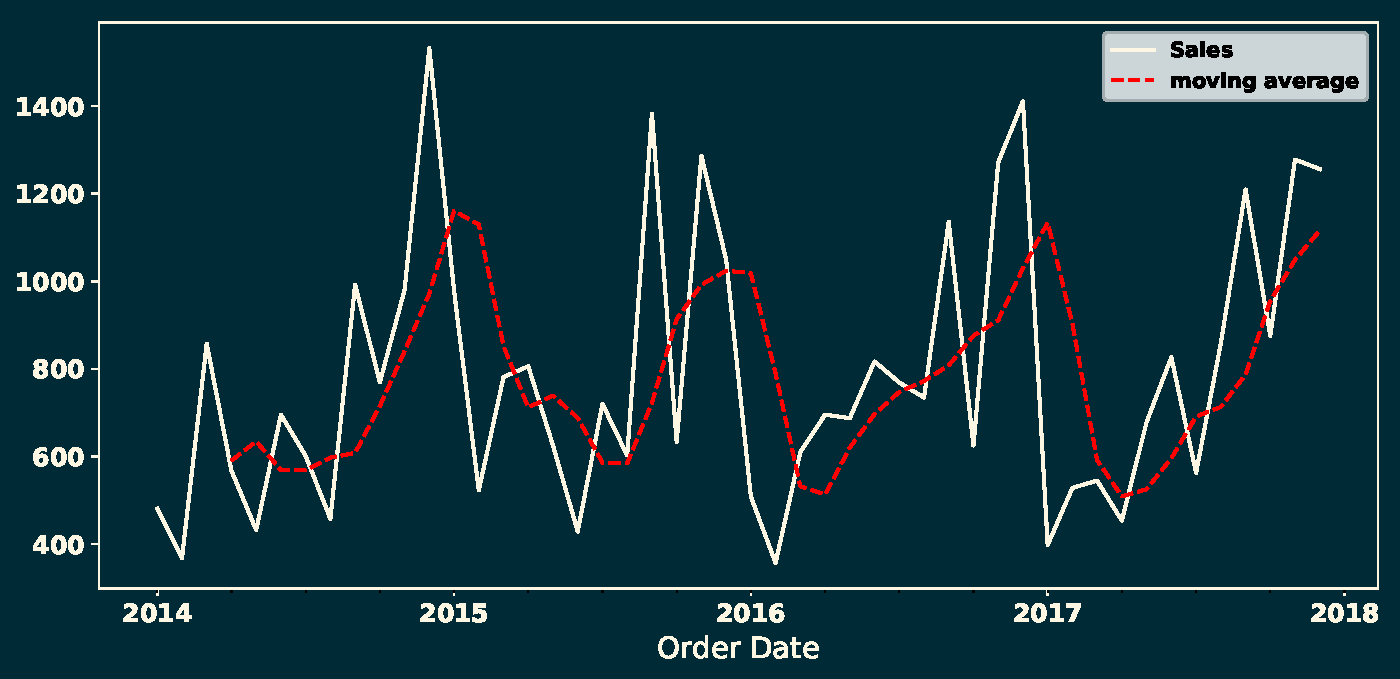
\includegraphics[width=\textwidth]{static/moving_average.pdf}
    \end{center}
\end{frame}

% \begin{frame}
%     \begin{center}
%     \textcolor{orange}{Autoregressive Integrated Moving Average (ARIMA)}
%     \end{center}
% \end{frame}

\begin{frame}
    \begin{center}
    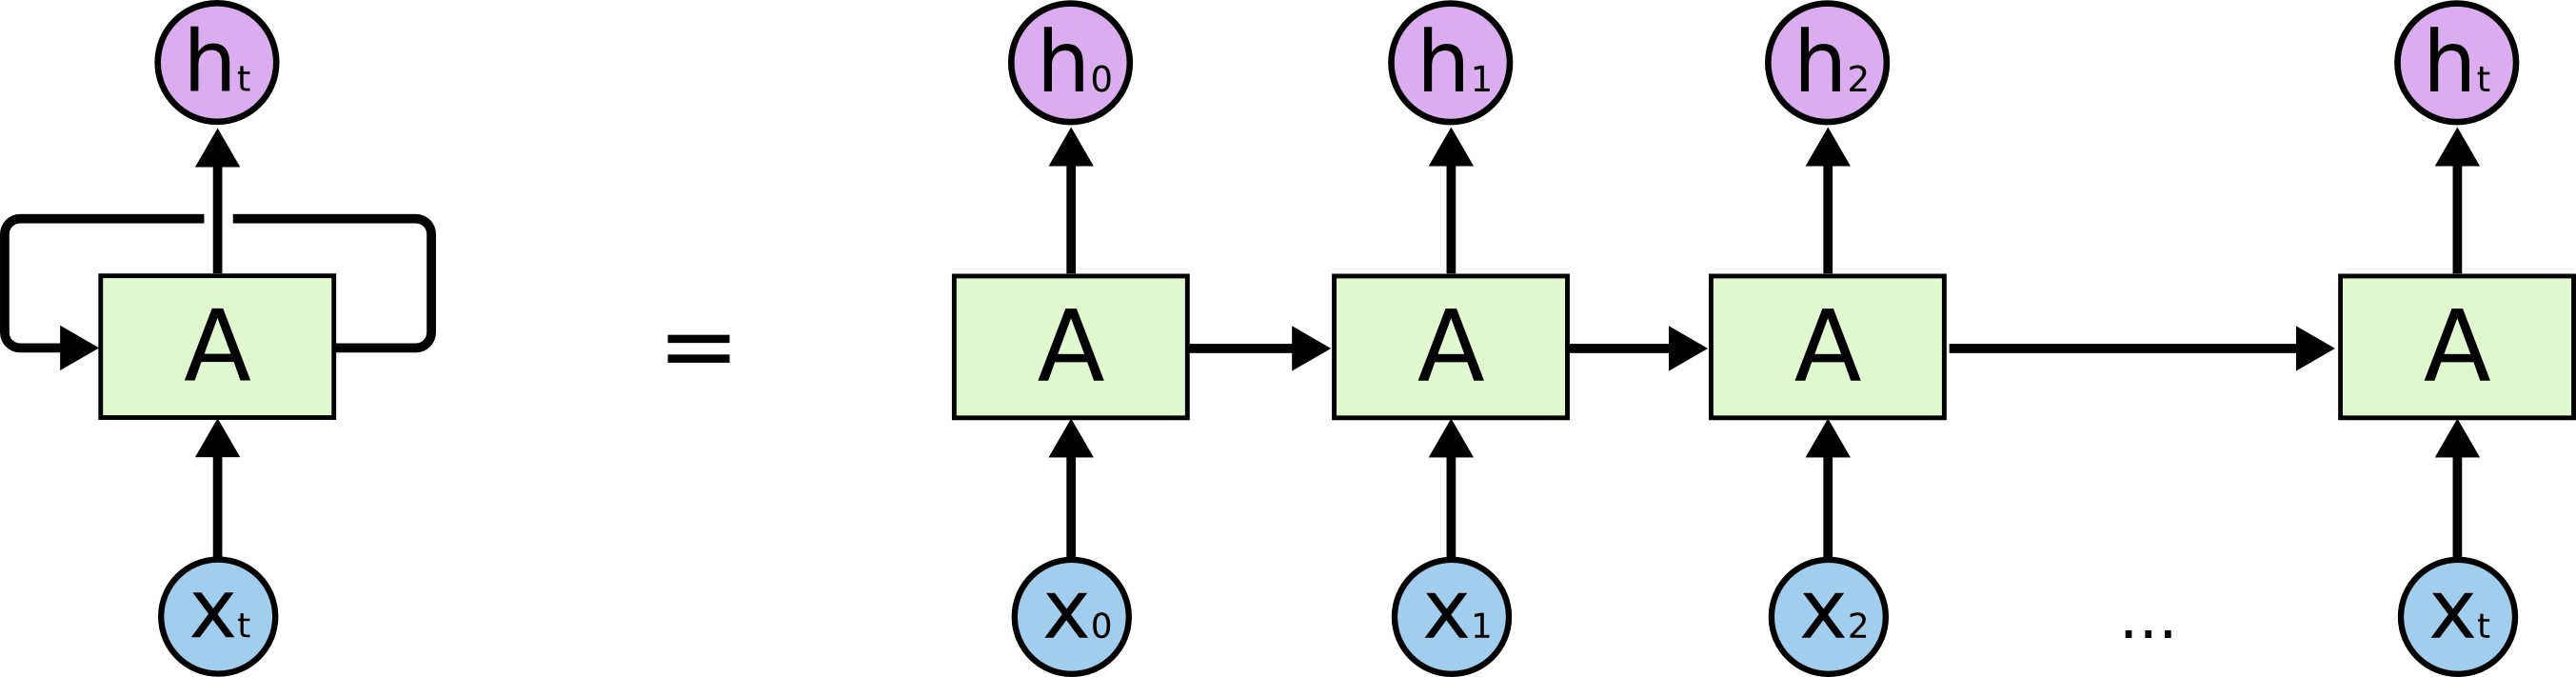
\includegraphics[width=\textwidth]{static/LSTM.png}\vspace{1cm}

    \small{https://colah.github.io/posts/2015-08-Understanding-LSTMs/}
    \end{center}
\end{frame}

\begin{frame}
    \begin{center}
    \Large \textcolor{orange}{\textbf{Python and R}}
    \end{center}
\end{frame}

\begin{frame}
    \begin{center}
    
\includegraphics[width=0.24\textwidth]{static/pydata.jpeg}\hspace{15pt}
    
\includegraphics[width=0.24\textwidth]{static/pydiff.png}\hspace{15pt}
    
\includegraphics[width=0.24\textwidth]{static/R.png}

    @pydatacardiff \qquad \quad @PyDiff \qquad \qquad @CardiffRUG

    \vspace{1cm}
    @NikoletaGlyn
    \end{center}
\end{frame}

\begin{frame}[fragile]
    \begin{columns}
        \begin{column}{.55\textwidth}
            \begin{minted}
                [
                framesep=4mm,
                baselinestretch=1.2,
                bgcolor=DarkGray,
                fontsize=\tiny,
                ]
                {python}
>>> import pandas
>>> nba = pandas.read_csv("nba_2013.csv")
        \end{minted}
        \end{column}
        \begin{column}{.55\textwidth}
            \begin{minted}
                [
                framesep=4mm,
                baselinestretch=1.2,
                bgcolor=DarkGray,
                fontsize=\tiny,
                ]
                {python}
> library(readr)
> nba <- read_csv("nba_2013.csv")
        \end{minted}
        \end{column}
    \end{columns}
\pause
\begin{columns}
    \begin{column}{.55\textwidth}
        \begin{minted}
            [
            framesep=4mm,
            baselinestretch=1.2,
            bgcolor=DarkGray,
            fontsize=\tiny,
            ]
            {python}
>>> train = nba.sample(frac=0.8, random_state=1)
>>> test = nba.loc[~nba.index.isin(train.index)]
    \end{minted}
    \end{column}
    \begin{column}{.55\textwidth}
        \begin{minted}
            [
            framesep=4mm,
            baselinestretch=1.2,
            bgcolor=DarkGray,
            fontsize=\tiny,
            ]
            {python}
> trainRowCount <- floor(0.8 * nrow(nba))
> set.seed(1)
> trainIndex <- sample(1:nrow(nba),
                     trainRowCount)
> train <- nba[trainIndex,]
> test <- nba[-trainIndex,]
    \end{minted}
    \end{column}
\end{columns}
\pause
\begin{columns}
    \begin{column}{.55\textwidth}
        \begin{minted}
            [
            framesep=4mm,
            baselinestretch=1.2,
            bgcolor=DarkGray,
            fontsize=\tiny,
            ]
            {python}
>>> from sklearn.linear_model import LinearRegression
>>> lr = LinearRegression()
>>> lr.fit(train[["fg"]], train["ast"])
>>> predictions = lr.predict(test[["fg"]])
    \end{minted}
    \end{column}
    \begin{column}{.55\textwidth}
        \begin{minted}
            [
            framesep=4mm,
            baselinestretch=1.2,
            bgcolor=DarkGray,
            fontsize=\tiny,
            ]
            {python}
> fit <- lm(ast ~ fg, data=train)
> predictions <- predict(fit, test)
    \end{minted}
    \end{column}
\end{columns}
\end{frame}

\end{document}

